% Questions-primary investigation map (poster pass): larger text, grounded equation terms.
% Six node classes distinguished; questions are the spine; one relation at the head.
% Compile: pdflatex -interaction=nonstopmode
\documentclass[border=16pt]{standalone}
\usepackage{amsmath}
\usepackage{tikz}
\usetikzlibrary{positioning,fit,backgrounds,calc,arrows.meta}

\definecolor{ink}{RGB}{45,55,70}
\definecolor{cLaw}{RGB}{238,240,244}
\definecolor{cQ}{RGB}{233,227,244}
\definecolor{tQ}{RGB}{96,70,150}
\definecolor{tSrc}{RGB}{42,84,140}
\definecolor{tTool}{RGB}{26,110,96}
\definecolor{tModel}{RGB}{150,104,20}
\definecolor{tFind}{RGB}{40,110,55}
\definecolor{note}{RGB}{105,105,115}

\newcommand{\sq}[1]{\textcolor{#1}{\rule{2.4mm}{2.4mm}}}

\begin{document}
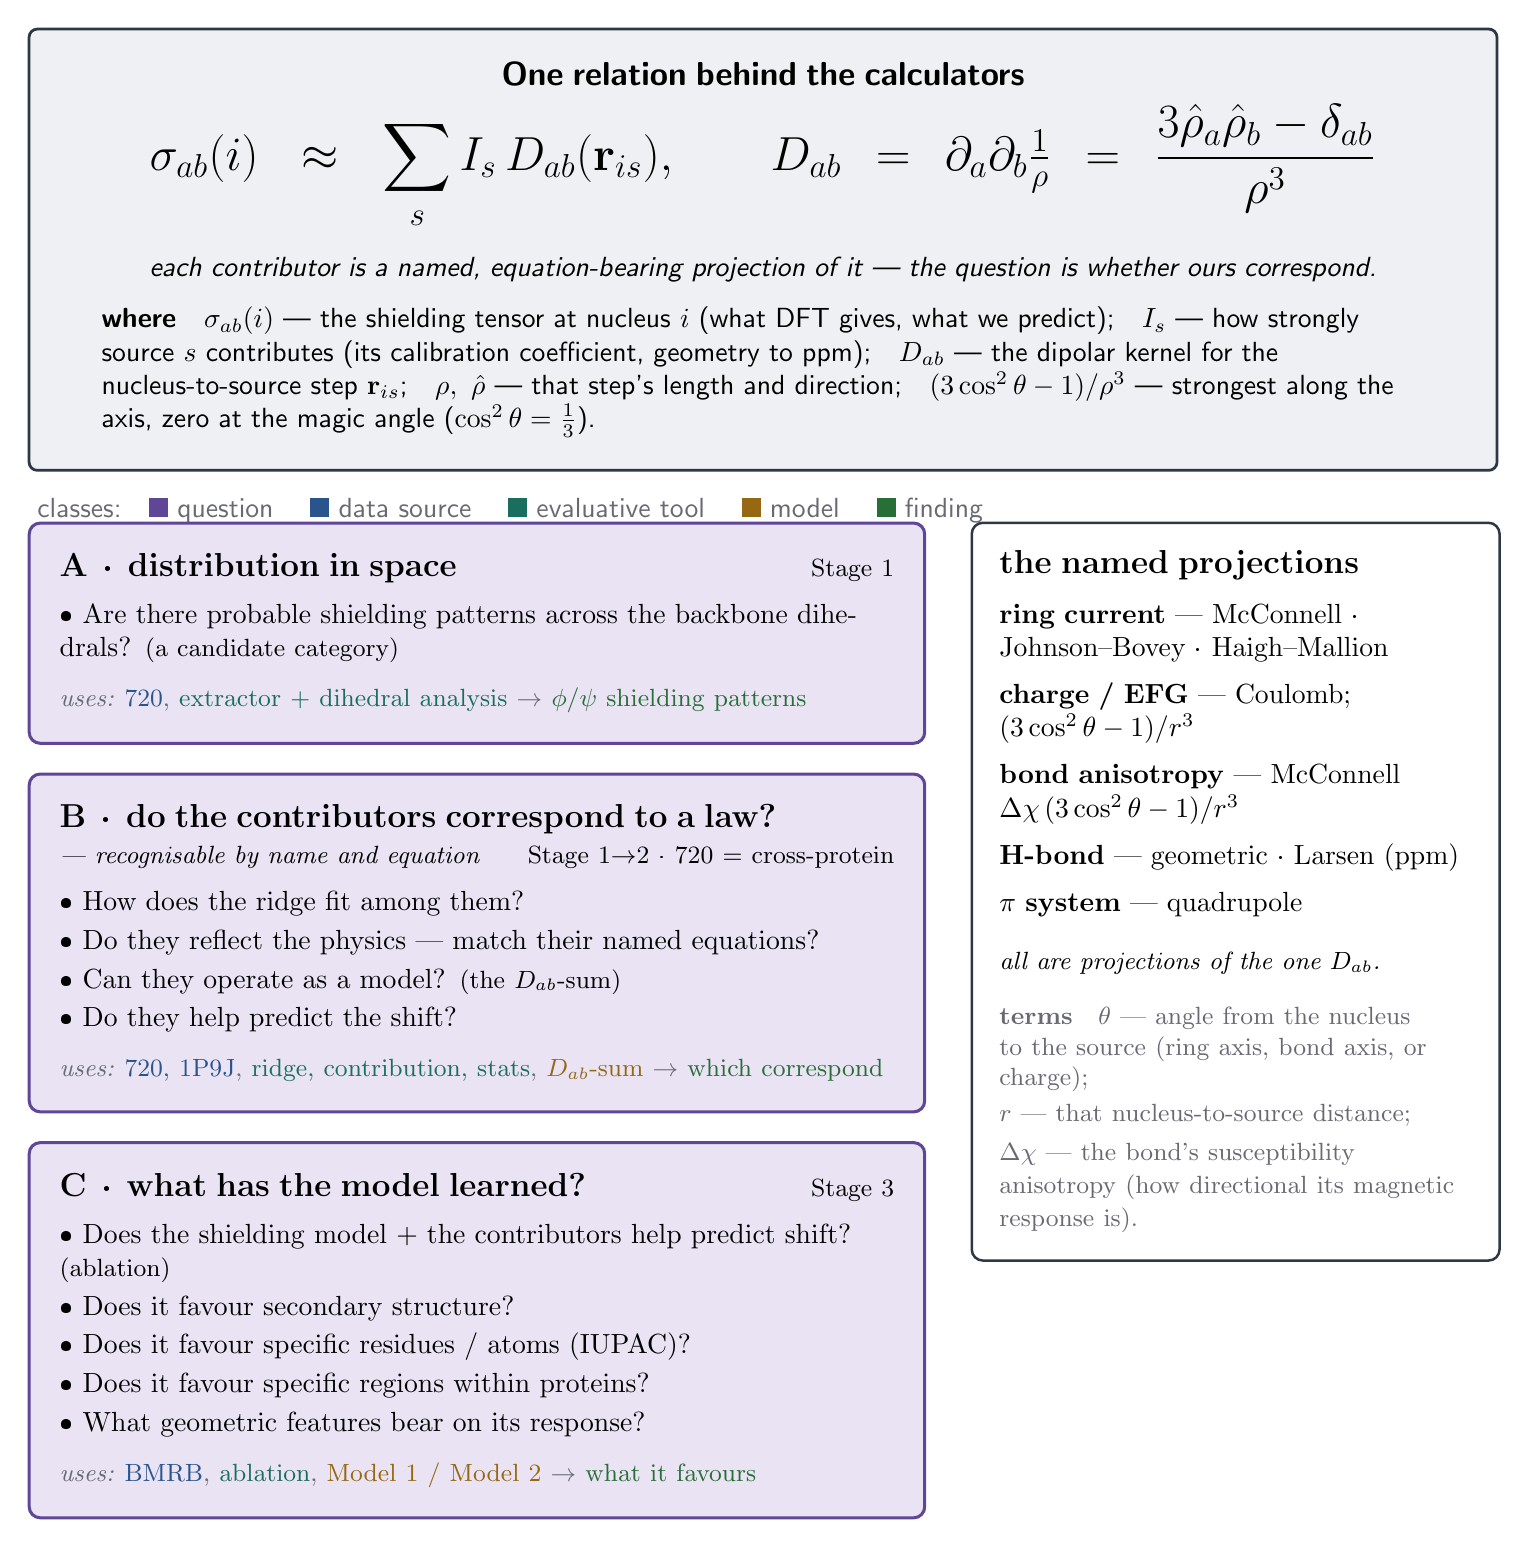
\begin{tikzpicture}[
  font=\sffamily,
  >={Stealth[length=2.4mm]},
  law/.style={rounded corners=3pt, draw=ink, line width=1pt, fill=cLaw, align=center, inner sep=12pt},
  grp/.style={rounded corners=4pt, draw=tQ, line width=1.1pt, fill=cQ, align=left, inner sep=11pt, text width=10.6cm, font=\normalsize},
  panel/.style={rounded corners=4pt, draw=ink, line width=0.9pt, fill=white, align=left, inner sep=10pt, text width=6.0cm, font=\normalsize},
]

% ---- the relation + grounded terms (head) ----
\node[law, text width=17.8cm] (LAW) at (0,0) {%
  {\large\bfseries One relation behind the calculators}\\[6pt]
  {\LARGE $\displaystyle \sigma_{ab}(i)\ \approx\ \sum_s I_s\, D_{ab}(\mathbf r_{is}),
   \qquad D_{ab}=\partial_a\partial_b\tfrac{1}{\rho}=\frac{3\hat\rho_a\hat\rho_b-\delta_{ab}}{\rho^{3}}$}\\[9pt]
  {\itshape each contributor is a named, equation-bearing projection of it --- the question is whether ours correspond.}\\[8pt]
  \begin{minipage}{16.8cm}\raggedright
   \textbf{where}\quad
   $\sigma_{ab}(i)$ --- the shielding tensor at nucleus $i$ (what DFT gives, what we predict);\quad
   $I_s$ --- how strongly source $s$ contributes (its calibration coefficient, geometry to ppm);\quad
   $D_{ab}$ --- the dipolar kernel for the nucleus-to-source step $\mathbf r_{is}$;\quad
   $\rho,\ \hat\rho$ --- that step's length and direction;\quad
   $(3\cos^2\theta-1)/\rho^3$ --- strongest along the axis, zero at the magic angle ($\cos^2\theta=\tfrac13$).
  \end{minipage}};

% ---- legend ----
\node[below=6pt of LAW.south west, anchor=north west, text=note] (LEG) {%
  classes:\quad \sq{tQ}~question \quad \sq{tSrc}~data source \quad \sq{tTool}~evaluative tool \quad \sq{tModel}~model \quad \sq{tFind}~finding};

% ---- question spine (left) ----
\node[grp, below=12pt of LEG.north west, anchor=north west] (A) {%
  {\large\bfseries A\, \textperiodcentered\, distribution in space}\hfill{\small Stage 1}\\[5pt]
  \textbullet\ Are there probable shielding patterns across the backbone dihedrals? {\small(a candidate category)}\\[6pt]
  {\small\color{note}\textit{uses:}\ \textcolor{tSrc}{720}, \textcolor{tTool}{extractor + dihedral analysis} $\to$ \textcolor{tFind}{$\phi/\psi$ shielding patterns}}};

\node[grp, below=10pt of A.south west, anchor=north west] (B) {%
  {\large\bfseries B\, \textperiodcentered\, do the contributors correspond to a law?}\\[1pt]
  {\small\itshape --- recognisable by name and equation}\hfill{\small Stage 1$\to$2 \textperiodcentered\ 720 = cross-protein}\\[5pt]
  \textbullet\ How does the ridge fit among them?\\[2pt]
  \textbullet\ Do they reflect the physics --- match their named equations?\\[2pt]
  \textbullet\ Can they operate as a model? {\small(the $D_{ab}$-sum)}\\[2pt]
  \textbullet\ Do they help predict the shift?\\[6pt]
  {\small\color{note}\textit{uses:}\ \textcolor{tSrc}{720, 1P9J}, \textcolor{tTool}{ridge, contribution, stats}, \textcolor{tModel}{$D_{ab}$-sum} $\to$ \textcolor{tFind}{which correspond}}};

\node[grp, below=10pt of B.south west, anchor=north west] (C) {%
  {\large\bfseries C\, \textperiodcentered\, what has the model learned?}\hfill{\small Stage 3}\\[5pt]
  \textbullet\ Does the shielding model + the contributors help predict shift? {\small(ablation)}\\[2pt]
  \textbullet\ Does it favour secondary structure?\\[2pt]
  \textbullet\ Does it favour specific residues / atoms (IUPAC)?\\[2pt]
  \textbullet\ Does it favour specific regions within proteins?\\[2pt]
  \textbullet\ What geometric features bear on its response?\\[6pt]
  {\small\color{note}\textit{uses:}\ \textcolor{tSrc}{BMRB}, \textcolor{tTool}{ablation}, \textcolor{tModel}{Model 1 / Model 2} $\to$ \textcolor{tFind}{what it favours}}};

% ---- named projections + their terms (right, spans the spine) ----
\node[panel, right=16pt of A.north east, anchor=north west] (NL) {%
  {\large\bfseries the named projections}\\[6pt]
  \textbf{ring current} --- McConnell \textperiodcentered\ Johnson--Bovey \textperiodcentered\ Haigh--Mallion\\[5pt]
  \textbf{charge / EFG} --- Coulomb; $(3\cos^2\theta-1)/r^3$\\[5pt]
  \textbf{bond anisotropy} --- McConnell $\Delta\chi\,(3\cos^2\theta-1)/r^3$\\[5pt]
  \textbf{H-bond} --- geometric \textperiodcentered\ Larsen (ppm)\\[5pt]
  \textbf{$\pi$ system} --- quadrupole\\[9pt]
  {\small\itshape all are projections of the one $D_{ab}$.}\\[9pt]
  {\small\color{note}\textbf{terms}\quad
   $\theta$ --- angle from the nucleus to the source (ring axis, bond axis, or charge);\\[2pt]
   $r$ --- that nucleus-to-source distance;\\[2pt]
   $\Delta\chi$ --- the bond's susceptibility anisotropy (how directional its magnetic response is).}};

\end{tikzpicture}
\end{document}
